\section{Introduction}
% We need to stare start with something with more punch
%r rather than just a f matter-of-fact statement
%Fair representations are a means of removing potentially sensitive information from training data
%in order to avoid wrongly relying on the sensitive information for classification.

Without due consideration for the data collection process, machine learning algorithms can exacerbate biases, or even introduce new ones if proper control is not exerted over their learning \citep{holstein2019improving}. 
While most of these issues can be solved by
% While efforts should be made to
controlling and curating data collection in a fairness-conscious fashion, 
% aiming to eliminate algorithmic bias during the early stages of the pipeline, 
doing so is not always an option, such as when working with historical data.
Efforts to address this problem algorithmically have been centred on developing statistical definitions of fairness and learning models that satisfy these definitions.
One popular definition of fairness used to guide the training of fair classifiers, for example, is \emph{demographic parity}, stating that positive outcome rates should be equalised (or \emph{invariant}) across protected groups.

In the typical setup, we have an input $\bm{x}$, a sensitive attribute $s$ that represents some non-admissible information like gender
and a class label $y$ which is the prediction target.
The idea of fair \emph{representation} learning \citep{zemel2013learning,edwards2016censoring,madras2018learning}
is then to transform the input $\bm{x}$ to a representation $\bm{z}$ which is invariant to $s$.
Thus, learning from $\bm{z}$ will not introduce a forbidden dependence on $s$.
% $\bm{z}$ can then be used to learn a predictor
% In fair representation learning \cite{zemel2013learning}\cite{edwards2016censoring}\cite{madras2018learning}, the goal is then to find a representation $\bm{z}$ that is invariant to $s$.
A good fair representation is one that preserves most of the information from $\bm{x}$ while satisfying the aforementioned constraints.
% While fair \emph{representations} are by no means the only method of achieving this goal, approaches that explicitly depend on the target label \cite{kamiran2012data} are restrictive in that they do not readily admit transfer to unseen tasks, and are bound by the requirement of having $s$ and $y$ labels be present together.

As unlabelled data is much more freely available than labelled data, it is of interest to learn the representation in an unsupervised manner.
This will allow us to draw on a much more diverse pool of data to learn from.
% ; this is particularly pertinent for fair representation learning as unlabelled data affords us a much more diverse pool of data to learn from.
%To this end, \cite{locatello2019fairness} recently made the connection from disentangled representations to fair representations:
%a model for disentanglement trained without knowledge of the sensitive attribute $s$
%nevertheless appears to improve fairness measures with respect to $s$.
%However, as pointed out by \cite{locatello2019challenging},
%some supervision or inductive bias is needed in order to recognise a well-disentangled representation.
While annotations for $y$ are often hard to come by (and often noisy; see~\cite{kehrenberg2020tuning}),
annotations for the sensitive attribute $s$ are usually less so, as $s$ can often be obtained from demographic information provided by census data.
We thus consider the setting where the representation is learned from data
that is only labelled with $s$ and not $y$.
This is in contrast to most other representation learning methods.
% We thus consider the setting where data labelled with $s$ (partially labelled data) is available for learning the fair representation.
% Furthermore, we assume the existence of a set with $s$ labels
% whose distribution matches the deployment setting
We call the set used to learn the representation the \emph{representative} set,
because its distribution is meant to match the distribution of the deployment setting
(and is thus representative).
% We call this set the \emph{representative} set and its distribution is meant to match the distribution of the deployment setting.

Once we have learnt the mapping from $\bm{x}$ to $\bm{z}$,
we can transform the \emph{training} set which, in contrast to the representative set, has the $y$ labels (and $s$ labels).
In order to make our method more widely applicable,
we consider an \emph{aggravated fairness problem}
% we allow the case
in which the training set contains a strong spurious correlation between $s$ and $y$,
which makes it impossible to learn from it a representation which is invariant to $s$ but not invariant to $y$.
Non-invariance to $y$ is important in order to be able to predict $y$.
The training set thus does \emph{not} match the deployment setting,
thereby rendering the representative set essential for learning the right invariance.
% We also tackle the related problem of learning from biased data, specifically cases in which the training set (with $y$ labels) contains a strong spurious correlation between $s$ and $y$, and thus does not match the deployment setting.
From hereon, we will use the terms \emph{spurious} and \emph{sensitive} interchangeably, depending on the context, to refer to an attribute of the data we seek invariance to.
% This is essentially a form of strong sampling bias and is not an unrealistic complication, having been shown to plague real-world datasets \cite{kallus2018residual}.
%Classifiers trained on ImageNet for example, have been shown to be biased towards texture \cite{Geir18}. \cite{zhang2018visual} similarly examine the problem of learning from biased data, showing that pre-trained models can exploit biases in the data by learning patterns semantically unrelated to the target, an issue that can be difficult to identify when the bias pervades both the training and test sets.
We can draw a connection between learning in the presence of spurious correlations and what \citet{kallus2018residual} call \emph{residual unfairness}.
Consider the Stop, Question and Frisk (SQF) dataset for example:
the data was collected in New York City, but the demographics of the recorded cases do not represent the true demographics of NYC well.
The demographic attributes of the recorded individuals might correlate so strongly with the prediction target that the two are nearly indistinguishable.
This is the scenario that we are investigating: $s$ and $y$ are so closely correlated in the labelled dataset that they cannot be distinguished, but the learning of $s$ is favoured due to being the ``path of least resistance''.
The deployment setting (i.e.\ the test set) does not possess this strong correlation and thus a na\"ive approach will lead to very unfair predictions.
In this case, a disentangled representation is insufficient;
the representation needs to be explicitly invariant solely with respect to $s$.
In our approach, we make use of the (partially labelled) representative set to learn this invariant representation.

While there is a substantial body of literature devoted to the problems of fair representation-learning, exactly how the invariance in question is achieved is often overlooked. 
When critical decisions, such as who should receive bail or be released from jail, are being deferred to an automated decision making system, it is critical that people be able to trust the logic of the model underlying it, whether it be via semantic or visual explanations. 
We build on the work of \citet{QuaShaTho19} and learn a decomposition ($f^{-1}: Z_s \times Z_{\neg s} \rightarrow X$) of the \emph{data domain} ($X$) into independent subspaces \emph{invariant} to  $s$ ($Z_{\neg s}$) and \emph{indicative} of $s$ ($Z_{s}$), which lends an interpretability that is absent from most representation-learning methods.
While model interpretability has no strict definition \citep{zhang2018visual}, we follow the intuition of \citet{adel2018discovering} -- \emph{a simple relationship to something we can understand}, a definition which representations in the data domain naturally fulfil.

Whether as a result of the aforementioned sampling bias or simply because the features necessarily co-occur, it is not rare for features to correlate with one another in real-world datasets.
Lipstick and gender for example, are two attributes that we expect to be highly correlated and to enforce invariance to gender can implicitly enforce invariance to makeup.
This is arguably the desired behaviour.
However, unforeseen biases in the data may engender cases which are less justifiable.
By baking interpretability into our model (by having representations in the data domain), though we still have no better control over what is learned, we can at least diagnose such pathologies.

To render our representations interpretable, we rely on a simple transformation we call \emph{null-sampling} to map invariant representations in the data domain.
Previous approaches to fair representation learning \citep{beutel2017data,edwards2016censoring,madras2018learning,louizos2016variational} predominantly rely upon autoencoder models to jointly minimise reconstruction loss and invariance.
We discuss first how this can be done with such a model that we refer to as cVAE (conditional VAE),
before arguing that the bijectivity of invertible neural networks (INNs)~\citep{Dinh2014} makes them better suited to this task. 
We refer to the variant of our method based on these as cFlow (conditional Flow).
INNs have several properties that make them appealing for unsupervised representation learning. 
The focus of our approach is on creating invariant representations that preserve the non-sensitive information maximally, with only knowledge of $s$ and not of the target $y$, while at the same time having the ability to easily probe what has been learnt.

% The problem of fair representations can also be viewed through a similar lens.
% A good toy model for this setup is the Coloured MNIST (cMNIST) dataset.
% In this example, the colour is a spurious variable which is very closely correlated with the prediction target in the training set but not in the deployment setting.
% An interpretable invariant representation in this case is the images uniform in colour. More details regarding the setup and synthesis of the dataset can be found in section~\ref{ssec:cmnist}.

% As a more real-world dataset, we consider the CelebA dataset.
% We treat the CelebA dataset as it is, as the deployment setting
% and construct deliberately biased subsets of CelebA to serve as the training set.
% In our experiments we use gender as the sensitive attribute.
% Sample images can be seen in \thomas{Fig.??}.
% Attributes that are correlated with gender in the \emph{deployment setting} (like the use of lipstick) will also be removed by our method.
% We do not consider this a defect of our method and instead argue that this is the correct behaviour:
% As long as the deployment setting is sufficiently diverse, the model may make use of correlations found in there.
%wearing lipstick is a valid indicator of gender.
%\thomas{maybe don't include the previous sentence}

Our contribution is thus two-fold:
1) We propose a simple approach to generating representations 
% through use of an INN, 
that are invariant to a feature $s$, while having the benefit of interpretability that comes with being in the data domain.
We call our model \emph{NIFR} (\emph{N}ull-sampling for \emph{I}nterpretable and \emph{F}air \emph{R}epresentations).
2) We explore a setting where the labelled training set suffers from varying levels of sampling bias,
% which we expect to be common not only in fairness problems but machine learning problems more broadly,
demonstrating an approach based on transferring information from a more diverse representative set,
with guarantees of the non-spurious information being preserved.

\begin{figure*}[tb]
  \centering
  \subfloat[Original images.]{%
      \scalebox{0.3}{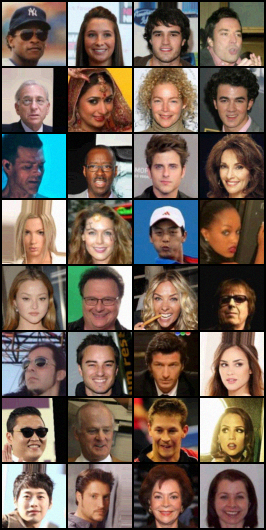
\includegraphics[width=\textwidth]{./Images/celeba/train_original_x_2.png}}%
      \label{fig:cflow_celeba_original_x}
  }
  \hfill
  \subfloat[$\bm{x}_u$ null-samples from the cFlow model.]{%
      \scalebox{0.3}{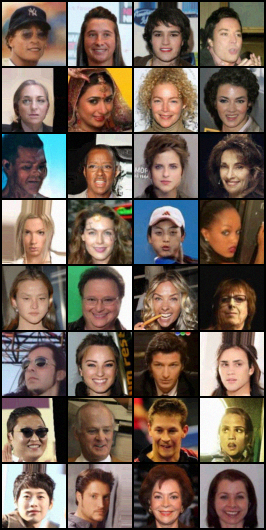
\includegraphics[width=\textwidth]{./Images/celeba/train_reconstruction_y_2.png}}%
      \label{fig:cflow_celeba_recon_y}
  }
  \hfill
  \subfloat[$\bm{x}_b$ null-samples from the cFlow model.]{%
      \scalebox{0.3}{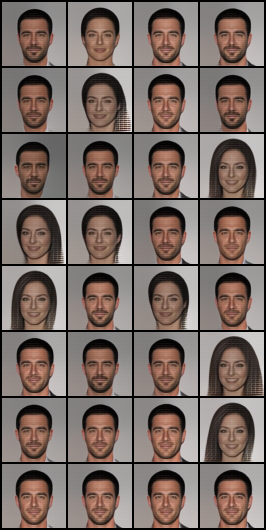
\includegraphics[width=\textwidth]{./Images/celeba/train_reconstruction_s_2.png}}%
      \label{fig:cflow_celeba_recon_s}
  }
  \caption{
    CelebA null-samples learned by our cFlow model, with gender as the sensitive attribute.
    (a) The original, untransformed samples from the CelebA dataset
    (b) Reconstructions using only information unrelated to $s$.
    (c) Reconstruction using only information related to $\neg s$.
    The model learns to disentangle gender from the non-gender related information.
    % Attributes such as \emph{makeup} and \emph{hair length} are also often modified in the process due to inherent correlations between them and the sensitive attribute, which the intepretability of our representations allows us to easily identify.
    Note that some attributes like skin tone seem to change along with gender due to the correlation between the attributes.
    This is especially visible in images (1,1) and (3,2). Only because our representations are produced in the data-domain can we easily spot such instances of entanglement.
  }%
  \label{fig:celeba_cflow}
\end{figure*}
